\section{Additional details}

% DG : cadre du cas opérateur (la 2nde hybridation n'utilise le DG que là) ; le corps ne présente que le CG
% \fcolorbox comme dans les anciennes présentations, coloré seulement à l'overlay 4 (cadre blanc avant, pour ne rien décaler)
\newcommand{\dgbox}[2]{\alt<3->{\fcolorbox{#1}{white}{$\displaystyle #2$}}{\fcolorbox{white}{white}{$\displaystyle #2$}}}
% étiquette de même couleur que son cadre, visible à l'overlay 4
\newcommand{\dglabel}[2]{\text{\uncover<3->{\textcolor{#1}{\footnotesize #2}}}}

\begin{frame}{Discontinuous Galerkin (DG) method\myfootcite{Arnold2002}}
	\appendixtarget{dg}
	\begin{minipage}[t]{0.62\linewidth}
		% \blk{1}{%
		For a \coloredonly<1>{fixed $\bm{\mu}\in\mathcal{M}$}, let $\mathcal{T}_h$ be a mesh of $\Omega$ of cells $(K_c)_{0\le c<N_\text{cells}}$.

		\vspace{5pt}

		Let $V_h^{\text{disc}}$ be a \coloredonly<1>{discontinuous space} of piecewise polynomials of \\
		degree $k$ on the mesh $\mathcal{T}_h$. Its basis functions $(\phi_{c,i})_{c,i}$, with $\phi_{c,i}$ \\
		supported on a single cell $K_c$, decompose the discrete solution:
		\vspace{-9pt}
		\[
			u_h(\bm{x},\bm{\mu}) = \sum_{c,i}\beta_{c,i}(\bm{\mu})\,\phi_{c,i}(\bm{x}).
		\]
		% }%
	\end{minipage} \hfill \begin{minipage}[t]{0.36\linewidth}
		\vspace{-6pt}
		\raggedleft
		\only<1>{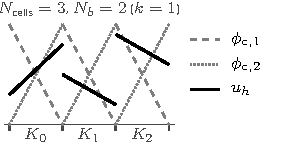
\includegraphics[page=1]{images/background/dg_basis/dg_basis.pdf}}%
		\only<2>{\includegraphics[page=2]{images/background/dg_basis/dg_basis.pdf}}%
		\only<3->{\includegraphics[page=3]{images/background/dg_basis/dg_basis.pdf}}
	\end{minipage}

	\vspace{3pt}
	\blk[until=2]{2}{%
		\textbf{Coupling the cells:} \coloredonly<2>{ambiguous traces on the interfaces $\Rightarrow$ numerical flux} (it defines the method)

		\vspace{5pt}

		Diffusion-dominated regimes: flux for the diffusion term only, here \coloredonly<2>{SIPG} (Symmetric Interior Penalty Galerkin)
	}

	\blk*{3}{%
	\textbf{Variational problem (SIPG):}

	Find $u_h\in V_h^{\text{disc}}$ such that, $\forall v_h\in V_h^{\text{disc}}$, $a_h^{\text{disc}}(u_h,v_h;\bm{\mu})=l(v_h;\bm{\mu})=\int_\Omega f\,v_h$, with

	\vspace{-3pt}
	\begin{equation*}
		\begin{aligned}
			a_h^{\text{disc}}(u_h,v_h;\bm{\mu}) =               & \qquad \dgbox{black!50}{\int_\Omega \Big(R\, u_h v_h + \bm{C}\cdot\gradh u_h\, v_h + \frac{1}{\text{Pe}} D\gradh u_h\cdot\gradh v_h\Big)} \; \raisebox{1.5ex}{$\dglabel{black!50}{cell terms}$} \\[-12pt]
			\raisebox{-2ex}{$\dglabel{orange}{consistency}$} \; & \; \dgbox{orange}{- \frac{1}{\text{Pe}}\int_{\mathcal{F}_h}\Big(\jump{u_h}\cdot\avg{D\gradh v_h} + \avg{D\gradh u_h}\cdot\jump{v_h}\Big)} \;
			\overset{\hspace{6em}\dglabel{red}{penalty}}{\dgbox{red}{+ \frac{1}{\text{Pe}}\int_{\mathcal{F}_h} \kappa\,\jump{u_h}\cdot\jump{v_h}}}
		\end{aligned}
	\end{equation*}

	where $\mathcal{F}_h$ is the set of faces, $\gradh$ the broken gradient, $\jump{\cdot}$ the jump, $\avg{\cdot}$ the average, $\kappa$ the penalty parameter.
	}
\end{frame}

\begin{frame}{Additional details}
	\todo[Détails de la méthode (hors présentation principale)]
\end{frame}

\section[Extra results]{Additional numerical results}
\begin{frame}{Additional numerical results}
	\todo[Résultats numériques supplémentaires]
\end{frame}
